While pipelines designs continue to improve, memory technology has been struggling to keep up with the increase in clock speed and performance.
Even though memory bandwidth can be improved with more bank parallelization, the memory latency remains the bottle neck to really improving memory performance.
Common memory technologies used in embedded systems contain a significant trade off between access latency and capacity. 
Static Random-Access Memories (SRAM) provides sufficient latency that allows single cycle memory access latencies from the pipeline.
However, the hardware cost to implement each memory cell prohibits large capacities to be implemented close to the processor.
On the other hand, Dynamic Random-Access Memories (DRAM) uses a compact memory cell design that can easily be designed into larger capacity memory blocks.
But the memory cell of DRAMs must be constantly refreshed due to charge leakage, and the large capacity of DRAM cells in a memory block design often prohibit faster access latencies.
%TODO: talk about about embedded systems seldom need disk?
To bridge the latency gap between the pipeline and memory, smaller memories are placed in between the pipeline and larger memories to act as a buffer, forming a memory hierarchy.
The smaller memories give faster access latencies at the cost of lower capacity, while larger memories make up for that with larger capacity but slower access latencies. 
The goal is to speed up program performance by placing commonly accessed values closer to the pipeline, while less access values are placed farther away.

\subsection{Memory Hierarchy}
\subsubsection{Caches}
\begin{wrapfigure}{r}{0.5\textwidth}
  \vspace{-20pt}
  \begin{center}
    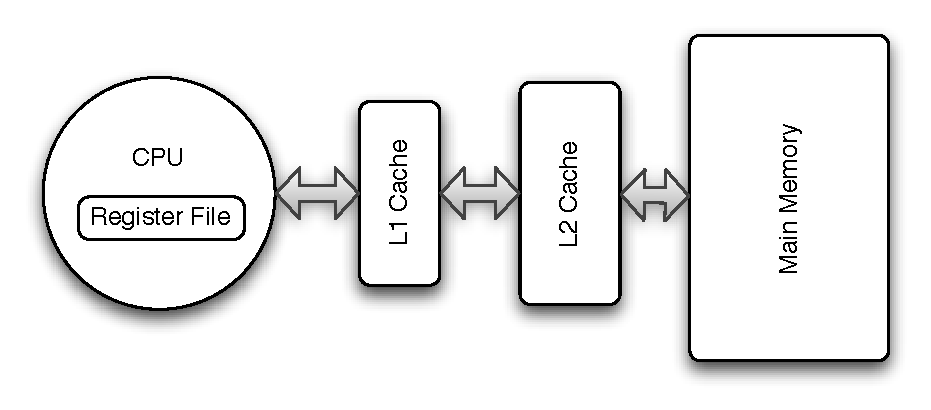
\includegraphics[scale=.5]{figs/conventional_mem_hierarchy}
  \end{center}
  \vspace{-20pt}
  \caption{Memory Hierarchy w/ Caches}
  \label{fig:conventional_mem_hierarchy}
  \vspace{-10pt}
\end{wrapfigure}   
A \emph{CPU Cache} (or cache) is commonly used in the memory hierarchy to manage the smaller fast access memory made of SRAMs.
The cache manages of contents of the fast access memory in hardware by leveraging the spatial and temporal locality of data accesses. 
The main benefits of the cache is that it abstracts away the memory hierarchy from the programmer.
When a cache is used, all memory accesses is routed through the cache. 
If the data from the memory access is on the cache, then a cache hit occurs, and the data is returned right away.
However, if data is not on the cache, then a cache miss occurs, and the cache controller fetches the data from the larger memory and adjusts the memory contents on the cache. 
The replacement policy of the cache is used to determine which cache line, the unit of memory replacement on caches, to replace. 
A variety of cache replacement policies have been researched~\todo{cite} and used to optimize for memory access patterns of different applications. 
In fact, modern memory hierarchies often contain multiple layers of hierarchy to balance the trade-off between speed and capacity.
A commonly used memory hierarchy is shown in figure~\ref{fig:conventional_mem_hierarchy}.
If the data value is not found in the L1 cache, then it is searched for in the L2 cache. 
If the L2 cache also misses, then the data is retrieved from main memory, and sent back to the CPU while the L1 and L2 cache updates its contents.
Often times different replacement policies are used at different levels of the memory hierarchy to optimize the hit rate or miss latency of the memory access.
Benchmarks have show that caches can have hit rates up to \todo{find number}\% \todo{and cite}. 

As sophisticated as this seems, the program is oblivious to the different levels of memory hierarchy, and whether or not an access hits the cache or goes all the way out to main memory. 
The memory hierarchy is abstracted away from the program, and the cache gives its best-effort to optimize memory access latencies.
This is one of the main reasons for the cache's popularity; the programmer does not need to put in extra effort to get a reasonable amount of performance.
A program can be run on any memory hierarchy configuration without modification and still obtain reasonable performance from the hardware.   
Thus, for general purpose applications, caches give the ability to improve design times and decrease design effort.
However, the cache makes no guarantees on actual memory access latencies and program performance. 
The execution time of programs could highly vary depending on a number different factors, cold starts, the execution context previously running, interrupt routines, and even branch mispredictions that cause unnecessary cache line replacements.  
Thus, when execution time is important, the variability and uncontrollability of caches may outweigh the benefits it provides. 

The cache uses internal states stored in hardware to manage the replacement of contents on it. 
As the programmer cannot control the states of the cache explicitly, it is extremely difficult to analyze the execution time of a program running with caches.
At an arbitrary point in the program, the state of the cache is unknown to the software.
Whether a memory access hits or misses the cache cannot to determined easily, so the conservative worst-case execution time analysis well need to assume the worst case as if the memory access was directly to main memory.
In theory, \todo{Cite and summarize Jan's thesis on cache analysis} showed that for certain cache replacement policies, it is possible to obtain tighter execution time analysis. 
However, the complexity of modern memory hierarchies with caches make timing analysis extremely difficult, and introduce high variability in program execution time.

Even outside of real-time applications, caches present side effects that it were not intended for.  
For applications that require extremely high speed, the best-effort memory management that caches offer simply is not good enough.
In those situations, programs need to be hand tuned and tailored to specific cache architectures and parameters.
Algorithm designers tune the performance of algorithms by reaching beneath the abstracted away memory architecture to enforce data access patterns to conform to the cache replacement policies and cache line sizes. 
Blocking~\cite{Lam91thecache}, for example, is a well-known technique to optimize algorithms for high performance.
Instead of operating on entire rows or columns of an array, algorithms are rewritten to operate on a subset of the data at a time, or blocks, so the faster memory in the hierarchy can be reused.
\todo{talk about LAPACK? Libraries that tune programs to caching}.
In this case, we see that the hidden memory hierarchy actually could degrade program performance.    
Multithreaded threaded architectures with shared caches amongst the hardware threads can suffer from \emph{cache thrashing}, an effect where different threads' memory accesses evict the cached lines of others.
In this situation, it is impossible for hardware threads have any knowledge on the state of the cache, because it is simultaneously being modified by other threads in the system. 
As a result, the hardware threads have no control over which level in the memory hierarchy they are accessing, and the performance highly varies depending on what is running on other hardware threads. 
For multicore architectures, caches create a data coherency problem when keeping data consistent between the multiple cores.
When the multiple cores are sharing memory, each core's private cache may cache the same memory address. 
If one core writes to a memory location that is cached in its private cache, then the other core's cache would contain stale data. 
Various methods such as bus snooping\todo{cite} or implementing a directory protocol\todo{cite} have been proposed to keep the data consistent in all caches. 
However, doing this scalably and efficiently is still a hot topic of research today\todo{cite all work on cache coherency}.

\subsubsection{Scratchpads}
We cannot argue against the need for a memory hierarchy, as there is an undeniable gap between processor and DRAM latency.
However, instead of abstracting away the memory hierarchy from the programmer, we propose to expose the memory layout to the software.  
\emph{Scratchpads} were initially proposed for their power saving benefits over caches\todo{cite}.
\todo{Papers that show scratchpads were already popular? Mention that they are already used. The Cell processor, Nvidia's 8800 GPU}
Scratchpads uses the same memory technology as caches, but does not implement the hardware controller to manage its memory contents.
Scratchpads have reduced access latency, area and power consumption compared to caches. 
Memory operations that access the scratchpad region take only a single cycle to complete, which is the same as a cache hit.
Thus, scratchpads may serve as the fast-access memory in a memory hierarchy, instead of caches. 
Unlike caches that overlay address space with main memory, scratchpads occupy a distinct address space in memory, so it does not need to check whether the data is on the scratchpad or not. 
Furthermore, the memory access time of each memory request is only depend on the memory address it is accessing. 
This drastically improves the predictability of memory access times, and reduces the variability of execution time introduced with caches.  
By using scratchpads, we explicitly expose the memory hierarchy to software, giving the programmer full control over the management of memory contents within the memory hierarchy.
\todo{show figure of memory hierarchy with scratchpads}

Two allocation schemes are commonly employed to manage the contents of scratchpads in software.
Static allocation schemes allocate data on the scratchpad during compile time, and the contents allocated on the scratchpad does not change throughout program execution. 
Static scratchpad allocation schemes~\cite{Suhendra2005WCETSPM, Patel2008PRETSPM} often use heuristics or compiler-based static analysis\todo{citation} of program to find the most commonly executed instructions or data structures, and allocate them statically on the scratchpad to improve program performance. 
Dynamic allocation schemes modify the data on the scratchpad during run time in software through DMA mechanisms.
The allocation could either be automatically generated and inserted by the compiler, or explicitly specified by the user programmatically.
Embedded system designs typically deal with limited resources and other design constraints, such as less memory or hard timing deadlines.    
Thus, the design of these systems often contain analysis on memory usage etc to ensure that the constraints are met. 
Actor oriented models of computations, such as Dataflow\todo{cite} or Giotto\todo{cite}, allow users to design systems at a higher level.
These higher level actor oriented programming models exposes the structure and semantics of the model for better analysis, which can be used to optimize scratchpad allocation dynamically.
Bandyopadhyay~\cite{Bandyopadhyay06_AutomatedMemoryAllocationOfActorCodeDataBufferInHeterochronous} presented an automated memory allocation of scratchpads for the execution of Heterochronous Dataflow models.
The Heterochronous Dataflow (HDF) model is an extension to the Synchronous Dataflow (SDF) model with finite state machines (FCM). 
The HDF models contain different program states, each state executing a SDF model that contains actors communicating with each other. 
Bandyopadhyay analyzed the actor code and the data that was being communicated in each HDF state.
The dynamic scratchpad allocation is inserted during state transitions, and the memory allocated is optimized for each HDF state. 
This allocation not only showed roughly 17\% performance improvement compared to executions using LRU caches, but also more predictable program performance.

The underlying memory technology that is used to make both scratchpads and caches is not inherently unpredictable, as SRAMs provide constant low-latency access time. 
However, caches manage the contents of the SRAM in hardware. 
By using caches in the memory hierarchy, the hierarchy is hidden from the programmer, and hardware managed memory contents creates highly variable execution times with unpredictable access latencies. 
Scratchpads on the other hand exposes the memory hierarchy to the programmer, allowing more predictable and repeatable memory access performances.
Although the allocation of scratchpads could be challenging, but it also provides opportunity for high efficiency, as it can be tailored to specific applications.   

\subsection{DRAM Memory Controller}
Because of its high capacity, DRAMs are often employed in modern embedded systems to cope with the increasing code and data sizes.  
However, bank conflicts and refreshes within the DRAM can cause memory accesses to stall, further increasing the memory latency. 
Modern memory controllers are designed to optimize average-case performance by queueing and reordering memory requests to improve throughput of memory requests. 
This results in unpredictable and varying access times and increased worst-case access time for each memory request.
In this section we will present a DRAM memory controller that privatizes DRAM banks with scheduled memory refreshes to provide improved worst-case latency and predictable access time.    
The contributions from this section is research done jointly with several co-authors from Reineke et. al~\cite{ReinekeLiuPatelKimLee11_PRETDRAMControllerBankPrivatizationForPredictability}. 
We do not claim sole credit for this work, and the summary is included in this thesis only for completeness purposes. 
We will first give some basic background on DRAM memories, then present the predictable DRAM controller designed.

\subsubsection{DRAM Basics}

\begin{figure}
\begin{center}
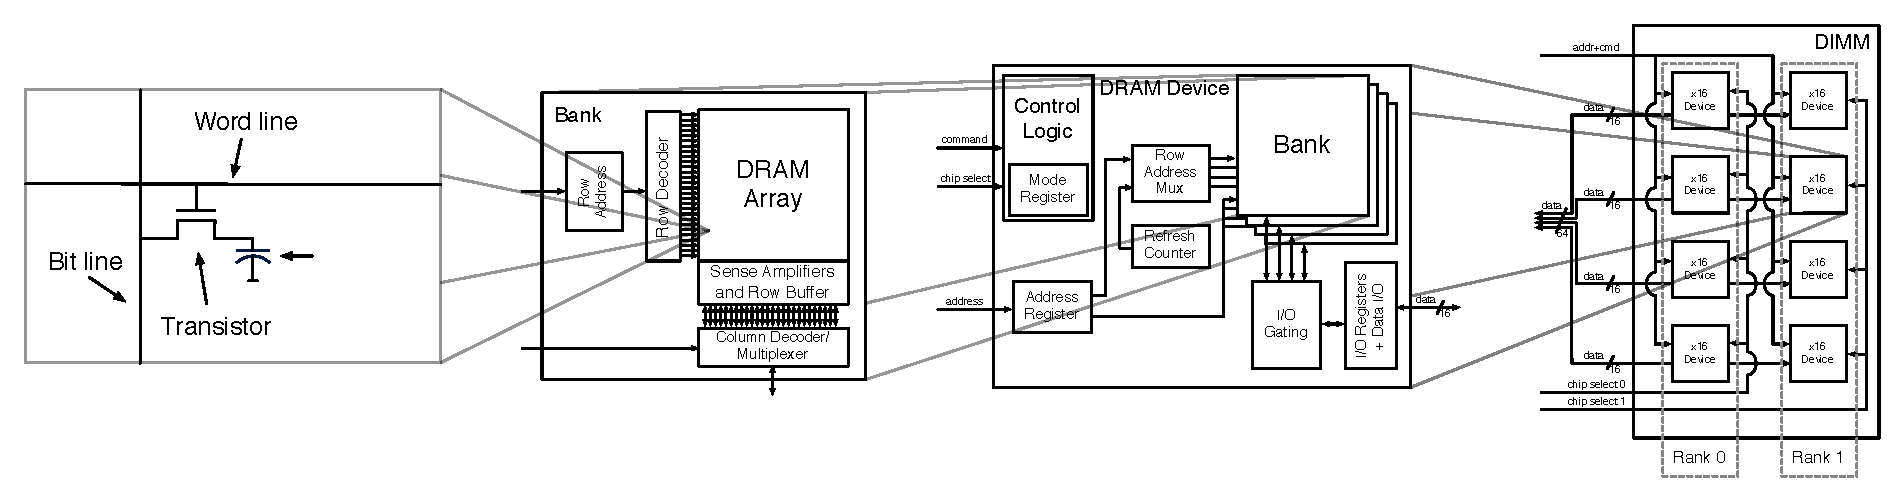
\includegraphics[width=\textwidth]{figs/dram-overview.pdf}
\vspace{-13mm}
\caption{A dual-ranked dual in-line memory module.}\label{fig:dram_basics}
\vspace{-6mm}
\end{center}
\end{figure} 

Figure~\ref{fig:dram_basics} shows the structure of a dual ranked in-line DDRII DRAM module.
Starting from the left, a basic \textbf{\emph{DRAM cell}} consists of a capacitor and a transistor. 
The capacitor charge determines the value of the bit, which can be accessed by triggering the transistor. 
Because the capacitor leaks charge, it must be refreshed periodically, typically every 64 ms or less~\cite{jedec}.
A \textbf{\emph{DRAM array}} is made of a two-dimensional array of DRAM cells.
Each access is made to the DRAM array goes through two phases: a row access followed by one or more column accesses.   
During the row access, one of the rows in the DRAM array is moved into the row buffer.
To read the value in the row buffer, the capacitance of the DRAM cells is compared to the wires connecting them with the row buffer.
The wires need to be precharged closed to the voltage threshold so the sense amplifiers can detect the bit value.
Columns can be read and written to quickly after the row is in the row buffer. 
The \textbf{\emph{DRAM device}} consists of banks formed of DRAM arrays. 
Modern DRAM devices have multiple banks, control logic, and I/O mechanisms to read from and write to the data bus as shown in the center of \ref{fig:dram_basics}.
Banks can be accessed concurrently, but the data, command and address busses are shared within the device, which is what the memory controller uses to send commands to the DRAM device. 
The following table\footnotemark lists the four most important commands and their function:
\footnotetext{This table is as shown in ~\cite{ReinekeLiuPatelKimLee11_PRETDRAMControllerBankPrivatizationForPredictability}}
%\begin{table}
\begin{center}
\begin{smalltabular}{p{13mm}p{6mm}p{10cm}}
Command 				& Abbr. & Description\\\hline
Precharge    			& PRE   & Stores back the contents of the row buffer into the DRAM array, and prepares the sense amplifiers for the next row access.\\
Row\hspace{13mm} access & RAS	& Moves a row from the DRAM array through the sense amplifiers into the row buffer.\\
Column access 			& CAS   & Overwrites a column in the row buffer or reads a column from the row buffer.\\
Refresh					& REF	& Refreshes several\footnotemark rows of the DRAM array. This uses the internal refresh counter to determine which rows to refresh.\\
\end{smalltabular}
%\caption{Overview of DDR2 Commands~\cite{ReinekeLiuPatelKimLee11_PRETDRAMControllerBankPrivatizationForPredictability}}
\label{tab:ddr2-commands}
\end{center}
%\end{table}
\footnotetext{The number of rows depends on the capacity of the device.}

To perform reads or writes, the controller first sends the PRE command to precharge the bank containing the data. 
Then, a RAS is issued to select the row, and one or more CAS commands can be used to access the columns within the row. 
Accessing columns from the same row does not require additional PRE and RAS commands, thus higher throughput can be achieved by performing column accesses in burst lengths of four to eight words.  
Column accesses can immediately be followed by a PRE command to decrease latency when accessing different rows. 
This is known as auto-precharge (or closed-page policy).
Refreshing of the cells can be done in two ways.
First, by issuing a refresh command, which refreshes all banks of the device simultaneously. 
The refresh latency depends on the capacity of the device, but the DRAM device manages a counter to step through all the rows.
The rows on the device could also be manually refreshed by performing row accesses to them.
Thus, the memory controller could performance row accesses on every row within the 64 ms refresh period.
This requires the memory controller to keep track of the refresh status of the device and issue more refresh commands, but each refresh takes less time because it is only a row access. 
\textbf{\emph{DRAM modules}} are made of several DRAM devices integrated together for higher bandwidth and capacity. 
A high-level view of the dual-ranked dual in-line memory module (DIMM) is shown in the right side of \ref{fig:dram_basics}.
The DIMM has eight DRAM devices that are organized in two ranks, which share the address, command and data bus. 
The two ranks share the address, command inputs, and the 64-bit data bus.
The chip is used to determine which ranks is addressed.
All devices within a rank are accessed simultaneously when the rank is addressed, and the results are combined to form the request response.  
% Due to the sharing of I/O mechanisms within a device, consecutive accesses to the same rank are more constrained than consecutive accesses to different ranks, which only share the command and address as well as the data bus.
% We later exploit this subtle difference by restricting consecutive accesses to different ranks to achieve more predictable access latencies.  
% We explain this in more detail in \ref{sec:pret_dram_controller}. 
Our controller makes use of a feature from the DDR2 standard known as posted-CAS.  
Unlike DDR or other previous versions of DRAMs, DDR2 can delay the execution of CAS commands (posted-CAS) for a user-defined latency, known as the additive latency ($AL$). 
Posted-CAS can be used to resolve command bus contention by sending the posted-CAS earlier than the corresponding CAS needs to be executed.

Table~\ref{table:ddr2-constraints} gives an overview of timing parameters for a DDR2-400 memory module.
These timing constraints come from the internal structure of DRAM modules and DRAM cells.
For example, $t_{RCD}, t_{RP}$, and $t_{RFC}$ are from the structure of DRAM banks that are accessed through sense amplifiers that need to be precharged.
$t_{CL}, t_{WR}, t_{WTR}$, and $t_{WL}$ result from the structure of DRAM banks and DRAM devices.
The four-bank activation window constraint $t_{FAW}$ constrains rapid activation of multiple banks which would result in too high a current draw.
The memory controller must conform to these timing constraints when sending commands to the DDR2 module.  
%The additive latency, $t_{AL}$, can be set by the user and determines how many cycles after a posted-CAS a CAS is executed.
Here we only gave a quick overview of DRAMs, we refer more interested readers to Jacob et al.~\cite{JaNgWa07} for more details.

\begin{table}
\begin{center}
\begin{smalltabular}{p{0.8cm}p{2.0cm}p{11cm}}
Para-meter	& Value (in cycles at 200 MHz)	& Description \\\hline
$t_{RCD}$			& 3						& Row-to-Column delay: time from row activation to first read or write to a column within that row.\\
$t_{CL}$			& 3						& Column latency: time between a column access command and the start of data being returned.\\
$t_{WL}$			& $t_{CL}-1=2$			& Write latency: time after write command until first data is available on the bus.\\
$t_{WR}$			& 3						& Write recovery time: time between the end of a write data burst and the start of a precharge command.\\
%$t_{CCD}$			& $\burstlength/2$ 				& CAS to CAS command delay. Minimum time between two read commands or two write commands.\\
$t_{WTR}$ 			& 2 					& Write to read time: time between the end of a write data burst and the start of a column-read command.\\% Allows the sense amplifiers to restore the data in the DRAM array.\\
$t_{RP}$			& 3						& Time to precharge the DRAM array before next row activation.  \\
%$t_{RTRS}$			& 1\todo{check this}	& Rank-to-rank switching time.\\ 
$t_{RFC}$			& 21					& Refresh cycle time: time interval between a refresh command and a row activation.\\
%$t_{REFI}$			& 1560    				& Refresh to refresh interval \\
%$t_{RAS}$ 			& $t_{RCD}+t_{WL}+t_{WR} = 8$ & Minimum time after an activate command to a bank until that bank is allowed to be precharged.\\
%$t_{RC}$			& $t_{RAS}+t_{RP}=11$	& Row cycle time: minimum time between successive activate commands to the same bank.\\
%$t_{RTP}$			&   			& Minimum time between a precharge command on a bank and a successive activate command.\\
$t_{FAW}$			& 10					& Four-bank activation window: interval in which maximally four banks may be activated.\\
$t_{AL}$			& set by user			& Additive latency: determines how long posted column accesses are delayed.
\end{smalltabular}
\vspace{-7.5mm}
%\todo{group constraints by their origin: constraints due to DRAM array structure, constraints due to sharing within DRAM device, constraints due to sharing of bus among ranks}
\end{center}
\caption{\small{Overview of DDR2-400 timing parameters of the Qimonda HYS64T64020EM-2.5-B2.~\cite{ReinekeLiuPatelKimLee11_PRETDRAMControllerBankPrivatizationForPredictability}}}\label{table:ddr2-constraints}
\end{table}

\subsubsection{Predictable DRAM Controller}
\label{sec:pret_dram_controller}
We will split the discussion of the predictable DRAM controller into its backend and frontend. 
The backend translates memory requests into DRAM commands that are sent to the DRAM module.
The frontend manages the interface to the pipeline along with the responsibility of scheduling the refreshes.
Here we specifically refer to a DDR2 667MHz/PC2-5300 memory module operating at 200Mhz, which has a total size of 512MB over two ranks with four banks on each rank.
While our discussion of the design of this DRAM controller is specific to our DDR2 memory module, the key design features are applicable to other modern memory modules.

\paragraph{Backend}
Conventional DRAM memory controllers view the entire memory device as one resource, and any memory requests can access the whole DRAM device. 
Subsequent memory accesses can target the same bank within the DRAM, which results in the need for memory requests to be queued and serviced sequentially, without exploiting bank parallelism.
Our controller views the memory devices as independent resource partitioned by banks. 
Specifically, we partition our memory module into four resources, each consisting of two banks within the same rank. 
The banks within each partition can be arbitrarily chosen, but all banks within a resource must belong to the same rank, and each of the ranks must contain at least two resources.
This is to avert access patterns that would incur high latency from the sharing of resources within banks and ranks.
The partitioning of the memory device allows us to fully exploit bank parallelism by accessing the resources in a periodic and pipelined fashion.
The periodic access scheme to the four resources interleaves each memory access between the ranks.
Subsequent accesses to the same rank go to different resources grouped from banks.  
Figure~\ref{fig:backend} shows an example of the following access requests: read from resource 0 in rank 0, write to resource 1 in rank 1, and read from resource 2 in rank 0. 

\begin{figure}
\begin{center}
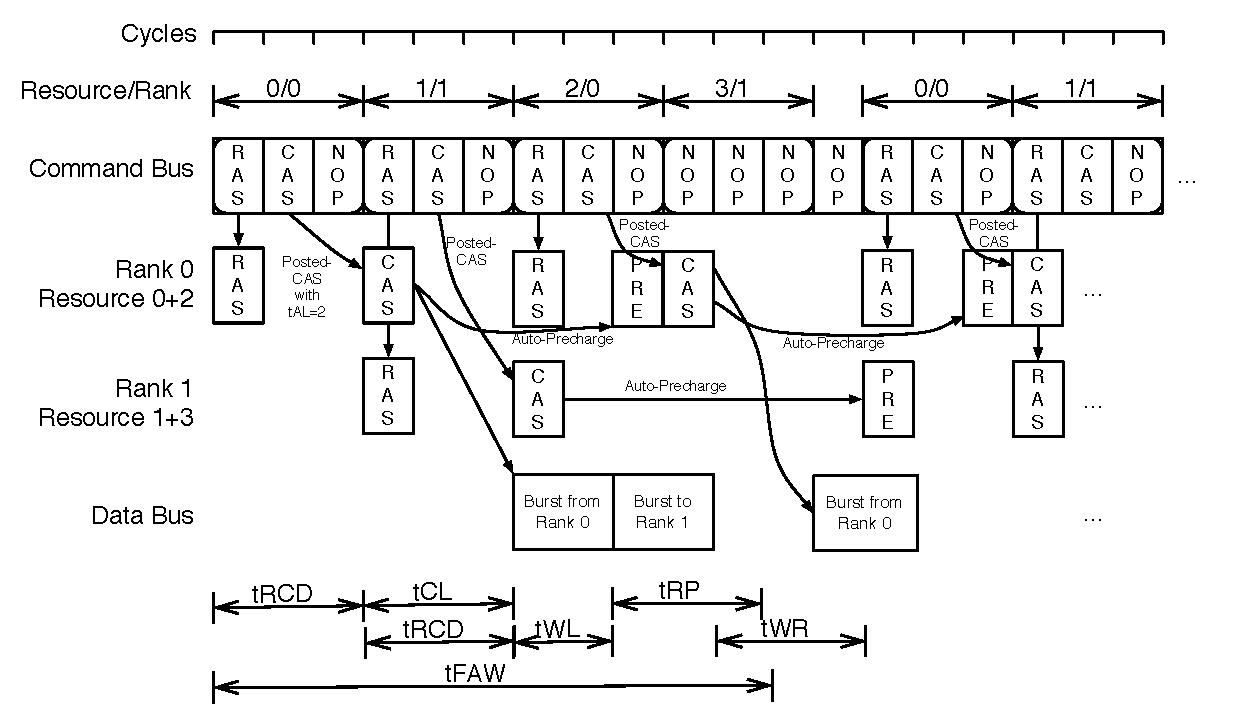
\includegraphics[width=0.92\linewidth]{figs/backend}
\end{center} 
\caption{\small{The periodic and pipelined access scheme employed by the backend~\cite{ReinekeLiuPatelKimLee11_PRETDRAMControllerBankPrivatizationForPredictability}.}}\label{fig:backend}
\end{figure}

Each access request is translated into a RAS (Row Access), posted-CAS (Column Access) and NOP command, which we call an access slot. 
The NOP command in the access slot is inserted between any two consecutive requests to avoid a collision on the data bus that occurs when a read request follows and a write request.
This collision is cause by the one cycle offset between the read and write latencies. 
The RAS command moves a row into the row buffer, and the CAS command accesses the columns within the row loaded into the row buffer. 
CAS commands can be either reads or writes, causing a burst transfer of $8 \cdot 4 = 32$ bytes that occupies the data bus for two cycles (as two transfers occur in every cycle).
We send a posted-CAS instead of a normal CAS in order to meet the row to column latency shown in \ref{table:ddr2-constraints}.
This latency specifies that the RAS command and the first CAS command need to be 3 cycles apart.  
However, figure~\ref{fig:backend} shows that manually issuing a CAS command to the first resource 3 cycles after its RAS command would cause a command bus conflict with the RAS command for the second resource.
Thus, we instead set the additive latency $t_{AL}$ to 2 and use the posted-CAS that offsets the CAS command to conform to the row to column latency.
This allows our memory controller to preserve our pipelined access scheme while meeting the latency requirements of the DRAM.   
We use a closed-page policy (also known as auto-precharge policy), which causes the accessed row to be immediately precharged after performing the column access (CAS), preparing it for the next row access.
If there are no requests for a resource, the backend does not send any commands to the memory module, as is the case for resource 3 in \ref{fig:backend}.

Our memory design conforms to all the timing constraints listed in table~\ref{table:ddr2-constraints}.
The write-to-read timing constraint $t_{WTR}$, incurred by the sharing of I/O gating within ranks, is satisfied by alternating accesses between ranks. 
The four-bank activation window constraint is satisfied because within any window of size $t_{FAW}$ we activate at most four banks within the periodic access scheme. 
Write requests with the closed-page policy requires 13 cycles to access the row, perform a burst access, and precharge the bank to prepare for the next row access.
However, our periodic access scheme has a period of 12 cycles, as each access slot is 3 cycles, and there are four resources accessed. 
Thus, a NOP is inserted after the four access slots: to increase the distance between two access slots belonging to the same resource from 12 to 13 cycles.
As a result, the controller periodically provides access to the four resources every 13 cycles.
The backend does not issue any refresh commands to the memory module.
Instead, it relies on the frontend to refresh the DRAM cells using regular row accesses.

% \paragraph{Longer Bursts for Improved Bandwidth}
% Depending on the application, bandwidth might be more important than latency.
% Bandwidth can be improved by increasing the burst length from 4 to 8.
% Extending the proposed access scheme to a burst length of 8 is straightforward with the insertion of two additional NOP commands after each request to account for the extra two cycles of data being transfered on the data bus.  
% In this case, the access slot latency for each request is increased from three to five to include the extra two NOP commands, and data will be transferred in four out of five cycles rather than in two out of three.
% Then, of course, latency of transfers of size less than or equal to 32 bytes increases, but the latency of large transfers decreases and higher bandwidth is achieved. 

\begin{wrapfigure}{r}{0.5\textwidth}
\begin{center}
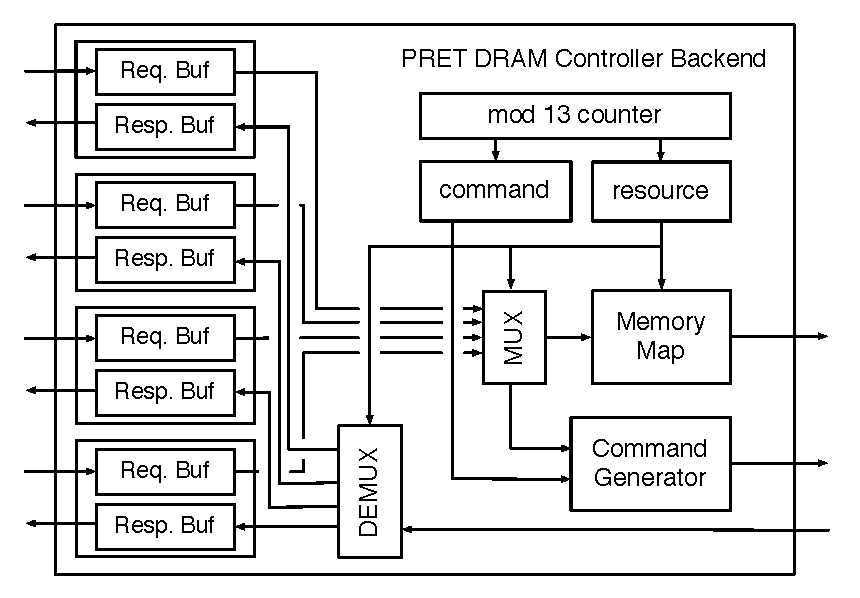
\includegraphics[width=1.1\linewidth]{figs/dram-backend-implementation}
\end{center}
\mycaption{\small{Sketch of implementation of the backend~\cite{ReinekeLiuPatelKimLee11_PRETDRAMControllerBankPrivatizationForPredictability}.}}\label{fig:dram-backend-implementation}
\end{wrapfigure}

A high level block view of our backend implementation is shown in figure~\ref{fig:dram-backend-implementation}.
Each resource has a single request buffer and a respond buffer.
These buffers are used to interface with the frontend.   
A request is made of an access type (read or write), a logical address, the data to be written for write requests. 
Requests are serviced at the granularity of bursts, i.e. 32 bytes in case of burst length 4 and 64 bytes in case of burst length 8.
A modulo-13 counter is used to implement the 13 cycle periodic access scheme in our controller.   
The ``resource'' and ``command" blocks are combinational circuits that are used to select the correct request buffer and generate the DRAM commands to be sent out. 
The ``memory map" block is where logical addresses are mapped to physical addresses that determine the rank, bank, row and column to access.
The data for read requests are latched into the response buffers to be read by the frontend.  

\paragraph{Frontend}
The frontend of our memory controller manages the interfacing to our backend, and the refreshing of the DRAM device.
The privatization of DRAM banks creates four independent resources that is to be accessed separately from the front end.
Thus, our memory controller is designed to be used by multicore or multithreaded architectures that contain multiple requesters which need access to the main memory.
Several recent projects strive to develop predictable multi-core architectures, such as those proposed by the MERASA~\cite{Ungerer10}, PREDATOR~\cite{Wilhelm09}, JOP~\cite{Schoeberl2008265}, or CoMPSoC~\cite{Hansson09} projects, which require predictable and composable memory performance.
These could potentially profit from using the proposed DRAM controller.
Specifically, we designed this memory controller to interface with the thread-interleaved pipeline discussed previously in section~\ref{section:pret_thread_pipeline}.
The thread-interleaved pipeline contains multiple hardware threads that each require access to main memory independently. 
We assign each hardware thread to a private memory resource, and send out memory requests to the memory controller frontend, which receives the request and places it within the request buffer.
Each thread in the thread-interleaved pipeline sends out only one outstanding memory request at a time, so the single request buffer for each resource is sufficient to interface with our thread-interleaved pipeline.
Once the request is serviced from the backend, the pipeline can read the data from the response buffer, and prepare to send another memory request.    
In section~\ref{sec:ptarm_memory} we will detail how our implemented thread-interleaved pipeline interfaces with this predictable DRAM controller, and discuss the memory access latency of this interaction.

The privatization of resources for predictable access means that there is no shared data in the DRAM.
This serves as an interesting design challenge, as it is impossible to assume no communication between contexts in a multicore or multithreaded environment.
In our implementation, which we will detail in section~\ref{sec:ptarm_memory}, we dedicate a region on the shared scratchpad that all the threads on our thread-interleaved pipeline can access in a single processor cycle.
This can be done because the scratchpad and DRAM memory has distinct address regions, so no shared memory space will overlap onto the DRAM. 
%If conventional caches were used, which can cache
However, most multi-core processors use DRAM to share data while local scratchpads or caches are private.
The sharing of data on the DRAM can be acheived by arbitrating accesses in the frontend.
In this case, the four resources in the backend can be combined into one, and any access to this single resource would result in four smaller accesses to all the backend resources. 
This single resource could then be shared among the different cores of a multi-core architecture using predictable arbitration mechanisms such as Round-Robin or CCSP~\cite{Akesson08} or predictable and composable ones like time-division multiple access (TDMA). 
This sharing of DRAM resources comes at a cost of increased memory access latency, which is detailed in~\cite{ReinekeLiuPatelKimLee11_PRETDRAMControllerBankPrivatizationForPredictability}. 

The frontend of our memory controller also manages the refreshing of DRAM cells. 
DRAM cells need to be refreshed at least every 64 ms.
Conventionally this is done by issuing a hardware refresh command that refreshes several rows of a device at once\footnote{Internally, this still results in several consecutive row accesses.}.
Hardware refresh commands have longer refresh latencies each time a refresh is issued, but requires less refresh commands to meet the refresh constraints posed by the DRAM.
However, when the hardware refresh command is issued, all banks in the target DRAM device are refreshed, prohibiting any other memory access to the device.
In our backend, this would extend across multiple resources, causing multiple resources to be blocked for memory accesses. 
Memory access latencies now need to account for potential refresh command latencies, which varies depending on the refresh progress.  
Instead, we use the distributed, RAS-only refresh~\cite{spec:micronddr2} to each bank separately.
Memory refreshes is in this case is equivalent to a row accesses to a bank, and each resource can be refreshed without effecting others.
Manually accessing rows on the other have much shorter latencies each time, but incurs a slight bandwidth hit because more accesses need to be performed to meet the refresh constraints.
The shorter latencies however improves the worst-case access latency, because the refresh latency is shorter.

When a refresh is required can be statically analyzed. 
In our device, each bank consists of 8192 rows, so each row has to be refreshed every $64\textit{ms}/8192=7.8125 {\mu}s$.
At a clock rate of 200 MHz of the memory controller, this corresponds to $7.8125 {\mu}s \cdot (200 \textit{cycles}/{\mu}s) = 1562.5$ cycles.
Since each resource contains two banks, we need to perform two refreshes every $1562.5$ cycles, or one every $781.25$ cycles.
One round of access is $13$ cycles at burst length 4, and includes the access slots to each resource plus a nop command. 
So in the frontend we schedule a refresh every $\lfloor 781.25/13 \rfloor^{th} = 60^{th}$ round of the backend.
If no memory access is in the request buffer for the resource being scheduled for refresh, then the row refresh can be directly be issued. 
Typically when a contention between a memory request and a refresh occurs, the refresh gets priority so the data can be retained in the DRAM cell. 
However, our refresh schedule schedules refreshes slightly more often than necessary.   
Scheduling a refresh every $60 \cdot 13$ cycles means that every row, and thus every DRAM cell, is refreshed every $60\cdot 13 \textit{ cycles}\cdot 8192\cdot 2/(200000~\textit{cycles}/\textit{ms}) \leq 63.90\textit{ms}$.
We can thus push back any of these refreshes individually by up to $0.1\textit{ms} = 20000$ cycles without violating the refreshing requirement.
So in our frontend, the memory request is serviced first (which takes 13 cycles), then the refresh is issued in the next access slot. 
In section~\ref{sec:ptarm_memory} when we detail the interaction between our thread-interleaved pipeline and the memory controller, we will show that the synchronization of the thread-interleaved pipeline to our controller backend allow us to completely hide memory refreshes in some unusable access slots lost in the synchronization.
Thus, providing predictable access latencies for all load/store instructions to the DRAM through our DRAM controller.

%\todo{discuss DMA?}
%We will also discuss interactions with DMA units    
%For loads sent from the pipeline, the pushed back refreshes become invisible:
%as the pipeline is waiting for the data to be returned and takes some time to reach the memory stage of the next instruction, it is not able to use successive access slots of the backend, and thus it is unable to observe the refresh at all.
%With this refresh scheme, refreshes do not affect the latencies of load/store instructions, and the refreshes scheduled within DMA transfers are predictable so the latency effects of the refresh can be easily analyzed.


